\documentclass{beamer}
\usepackage{listings}
\lstset{
%language=C,
frame=single, 
breaklines=true,
columns=fullflexible
}
\usepackage{subcaption}
\usepackage{url}

\usepackage{tikz}
\usepackage{pgfplots}
\pgfplotsset{compat=1.17}
\usepackage{tkz-fct}
\usepackage{mathrsfs}
\usepackage{txfonts}
\usepackage{tkz-euclide} 
\usetikzlibrary{calc,math}
\usepackage{float}
\newcommand\norm[1]{\left\lVert#1\right\rVert}
\renewcommand{\vec}[1]{\mathbf{#1}}
\providecommand{\pr}[1]{\ensuremath{\Pr\left(#1\right)}}
\usepackage[export]{adjustbox}
\usepackage[utf8]{inputenc}
\usepackage{amsmath}
\usetheme{Boadilla}
\title{Low Reliable and Low Latency Communications for Mission Critical Distributed Industrial Internet of Things}
\author{Digjoy Nandi - AI20BTECH11007}

\begin{document}
\begin{frame}
\titlepage
\end{frame}
\section{Introduction}
\begin{frame}{Keywords and some definitions}
\begin{block}{Reliablity}
  Reliability is defined as the probability that a product, system, or service will perform its intended function adequately for a specified period of time, or will operate in a defined environment without failure.
\end{block}
    \begin{block}{Latency}
   Latency from a general point of view is a time delay between the cause and the effect of some physical change in the system being observed.
    \end{block}
    \begin{block}{Internet of things(LoT)}
     The Internet of things describes the network of physical objects/"things"—that are embedded with sensors, software, and other technologies for the purpose of connecting and exchanging data with other devices and systems over the Internet.
    \end{block}

\end{frame}
\begin{frame}{}
\begin{block}{Consensus}
    Consensus decision-making is group decision-making processes in which participants develop and decide on proposals with the aim, or requirement, of acceptance by all.

\end{block}
\begin{block}{Q-function}
    In statistics, the Q-function is the tail distribution function of the standard normal distribution. In other words, Q(x) is the probability that a normal (Gaussian) random variable will obtain a value larger than x standard deviations.
    \begin{equation}
        Q(x)=P(X>x)
    \end{equation}
    where, $$x=\frac{x-\mu}{\sigma}$$
    It is a decreasing monotonous function.

\end{block}

\end{frame}
\begin{frame}{Centralised v/s Distributed consensus system}
\begin{block}{Motive:}
In some critical IIoT application scenarios, URLLC needs to provide an end-to-end latency lower than 1 ms and exceedingly high reliability more than$ 1-10^9$

\end{block}
\begin{figure}
    \centering
    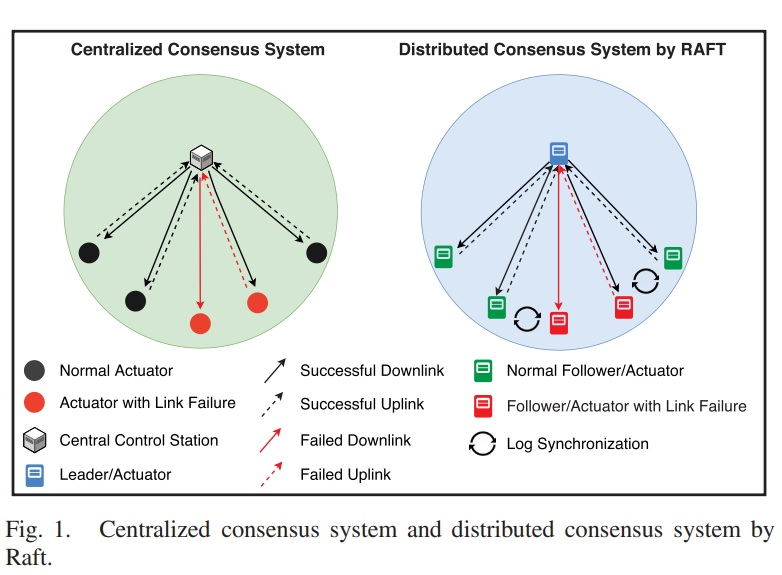
\includegraphics[width = 1\columnwidth ]{Untitled.jpg}
\end{figure}
\end{frame}
\section{Raft Algorithm}
\begin{frame}{Raft}
There are three roles in Raft algorithm.
\begin{figure}
    \centering
    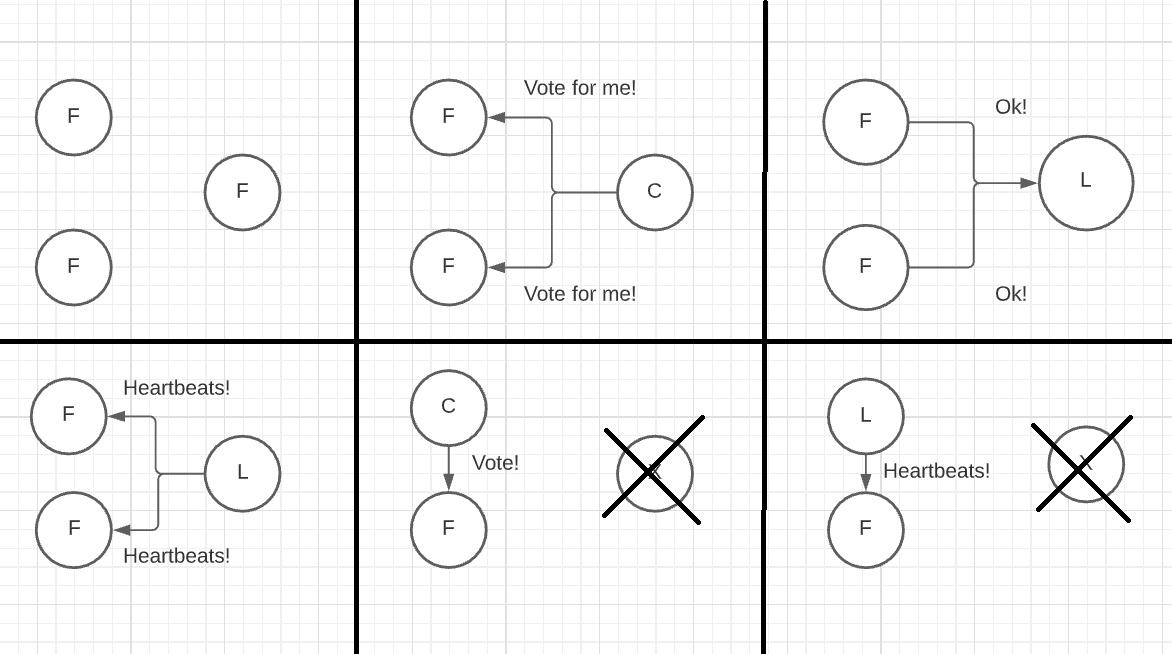
\includegraphics[width = 1\columnwidth]{edit.jpg}
    \caption{Election of a leader}
\end{figure}

\end{frame}
\begin{frame}{Log Replication}
\begin{figure}
    \centering
    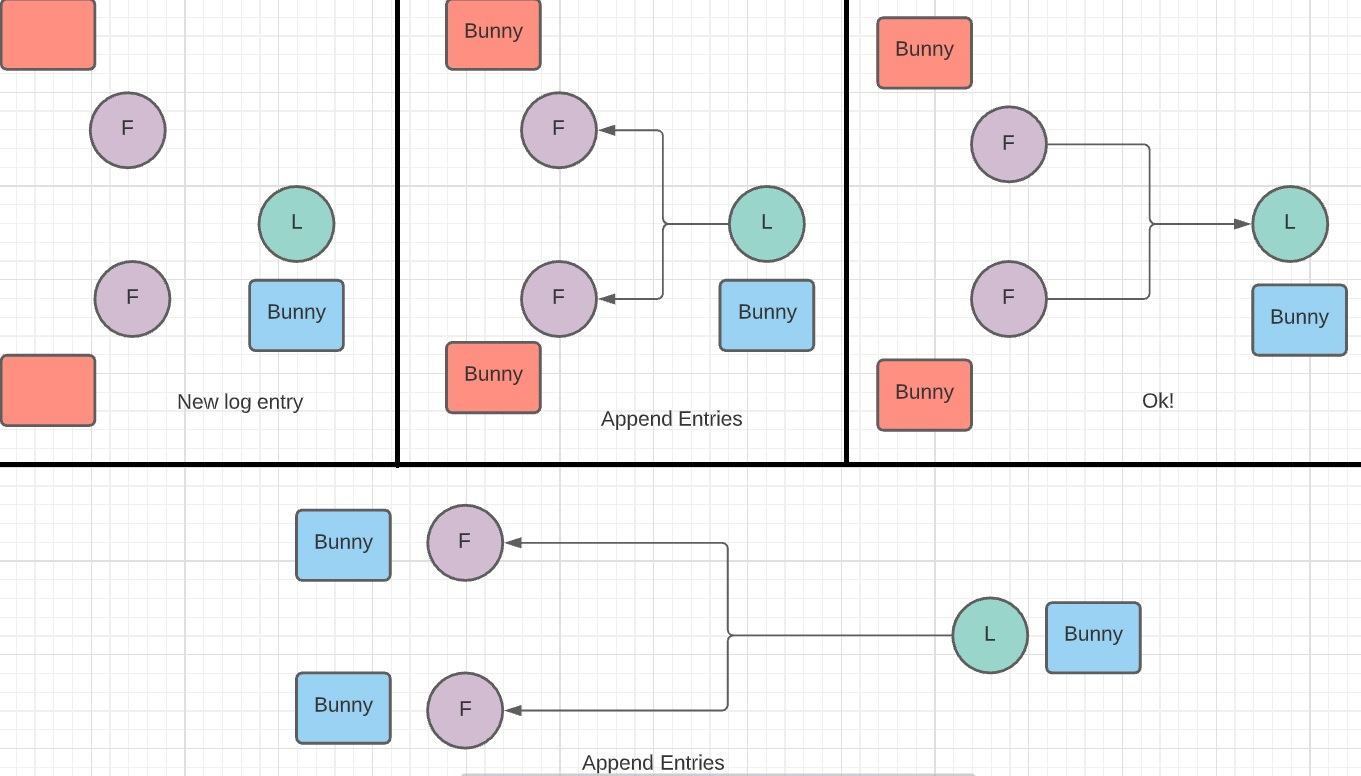
\includegraphics[width = 1\columnwidth]{log.jpg}
    \caption{Log Replication}
\end{figure}
    
\end{frame}

\section{Reliability}
\begin{frame}{Reliability of Communication System With Raft}
\begin{enumerate}
  \item
    Let us consider N nodes in a distributed system with
Raft CM
  \item 
  A reliable critical decision requires that over $\frac{N-1}{2}$ followers who can receive log entries from the leader and send the confirmed messages back to the leader to achieve the commitment of log replication.
  \item
  It is worth to mention that 50$\%$ is the fault tolerance of Raft.
\end{enumerate}
\end{frame}
\begin{frame}{Reliability of Communication System With Raft}
\begin{block}{Consensus success rate}
    Let $P_{l}$ be communication link success rate and $P_{C}$ be consensus success rate of the system.
    \begin{equation}
        P_C=\displaystyle\sum_{i=\frac{N-1}{2}}^{N-1}{i \choose N-1} P_{l}^{i} (1-P_{l})^{N-1-i} \times \displaystyle\sum_{j=\frac{N-1}{2}}^{i}{j \choose r} P_{l}^{j} (1-P_{l})^{i-j}
    \end{equation}
\end{block}
\end{frame}

\begin{frame}{Reliability of Communication System With Raft}
\begin{block}{}
    \begin{enumerate}
     \item 
     The first summation represents the probability that the majority of followers can download the  log entry from the leader.
     \item
     The second summation equals to the probability that the majority of followers can upload their confirmation back to the leader.
     \item
     The number of successful uplink transmission is never larger than the number of successful downlink transmissions.
    \end{enumerate}
\end{block}
\begin{block}{Note}
According to the (2), to satisfy the most stringent reliability requirement in IIoT, i.e., the consensus failure rate $1-P_C$ is less than $10^{-9}$, the nodes number N should not be less than 69, 31, 12, 5, when the link success rate $P_l$ is 90$\%$, 95$\%$, 99$\%$ and 99.9$\%$, respectively.
\end{block}
\end{frame} 
\begin{frame}{Reliability Gain}
\begin{block}{Reliability Gain}
Reliability Gain is a parameter (also can be interpreted as reliability amplification factor) to represent the quantitative relationship between the reliabilities of consensus and communication link.
\begin{equation}
    log(1-P_C)= klog(1-P_l) + h
\end{equation}
where, reliability gain,$k=\frac{N+1}{2}$ and intercept $h=log\left({{\frac{N-3}{2}}\choose{ N-1}}\right)+\triangle h$
\end{block}    
\end{frame}
\begin{frame}{Reliability Gain}
\begin{block}{}
\begin{enumerate}
    \item 
    The consensus failure rate and link failure rate are in linear relation when the nodes number N is constant.
    \item
     With fixed link reliability, the increasing nodes number rises up the consensus reliability, which proves the increasing monotonicity of consensus success rate $P_C$ with the nodes number N.
\end{enumerate}
\end{block}
\begin{figure}
    \centering
    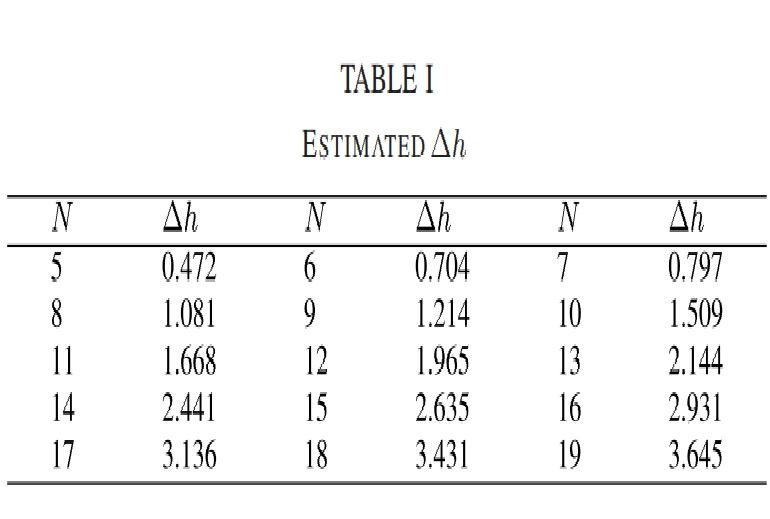
\includegraphics[scale=0.5]{h.jpg}
\end{figure}
\end{frame} 
\section{Latency}
\begin{frame}{Relationship Between Latency and Reliability}
 \begin{block}{}
 \begin{enumerate}
     \item 
     Let us consider a wireless communication model, which aims to analyze the packet error probability of the wireless short package transmissions in URLLC, to find out the relationship between consensus success rate $P_C$ and the consensus latency T.
     \item 
     We assume it is caused by downlink and uplink transmission delay, i.e., Raft consensus latency T only composes of communication transmission delay to show the communication impacts on the overall consensus latency.
     \item
     The link failure rate can be written as function as T as follows.
     \begin{equation}
         1-P_l =f_{Q}\left(\frac{B\frac{T}{2N}(C-R)+\frac{\log_{2}(B\frac{T}{2N})}{2}}{(B\frac{T}{2N})^{1/2}\log_{2}e}\right) 
     \end{equation}
 \end{enumerate}
 
\end{block}
     
\end{frame}
\begin{frame}{Relationship Between Latency and Reliability}
 \begin{enumerate}
     \item 
     B is the available spectrum bandwidth.
     \item
     R and C are the uplink or downlink transmission rate and channel capacity, respectively.
 \end{enumerate}
 \begin{block}{Note}
The overall consensus delay, T , each transmission can have
$t =\frac{T}{2N}$ transmission internal since there are N transmissions in both uplink and downlink. Therefore, with a constant N, the increasing consensus delay T can provide more time t for each link transmission, which intuitively can reduce the link failure rate $1 - P_{l}$.

\end{block} 
 \end{frame}
\begin{frame}{Relationship Between Latency and Reliability}
 \begin{block}{Latency and Reliability}

 \begin{enumerate}
     \item
    By substituting equation(4) into (2) or (3), we can obtain the relationship of reliability $1-P_C$ with the latency T .
    \item
    The contradiction of consensus reliability $1-P_C$ and time delay T can be proved in mathematics by calculating the derivative of the variable Q in Q function.
    \begin{equation}
        \frac{\delta Q}{\delta T}=\frac{\frac{B}{2N}(C-R)-\frac{1}{2T}\log_{2}(\frac{TB}{2N})+\frac{1}{T}(\log_{e}2)}{2\sqrt{\frac{TB}{2N}}\log_{2}e} 
    \end{equation}
\end{enumerate}
\end{block}
\end{frame}
\begin{frame}{Relationship Between Latency and Reliability}
 \begin{block}{Latency and Reliability}

 \begin{enumerate}
     \item
    The derivative $\frac{\delta Q}{\delta T}$ is always positive,which means the variable increases monotonically along with T.
     \item
    Based on the decreasing monotonicity of Q-function $f_{Q}$ along with Q and the increasing monotonicity of $P_C$ along with $P_l$, the time delay of consensus T and consensus reliability $1 - P_C$ are contradictory.
 \end{enumerate}
\end{block}
\end{frame}

\begin{frame}{Relationship Between Latency and Reliability}
 \begin{block}{Conclusion}

 \begin{enumerate}
     \item
    The consensus reliability $1 - P_C$ increases monotonically with the nodes number.
     \item
    However, given fixed consensus delay T , increasing node number will also result in a shorter transmission time t =$\frac{T}{2N}$ for each link.
     \item 
    Thus causing a smaller $P_l$, which may turn out a less reliable consensus according to equation (2) or (3). Thus, it is expected that there is an optimal N to achieve maximum consensus reliability.
 \end{enumerate}
\end{block}
\end{frame}

\begin{frame}{Simulation Results}
\begin{figure}
    \centering
    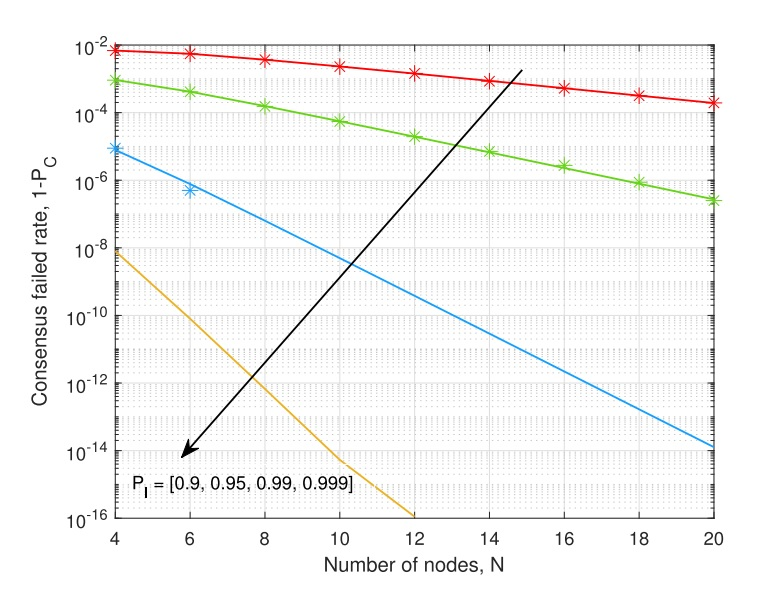
\includegraphics[scale=0.5]{PC.jpg}
    \caption{Consensus failure rate $1-P_C$ vs. Nodes number N}
\end{figure}


\end{frame}
\begin{frame}{Simulation Results}
\begin{figure}
    \centering
    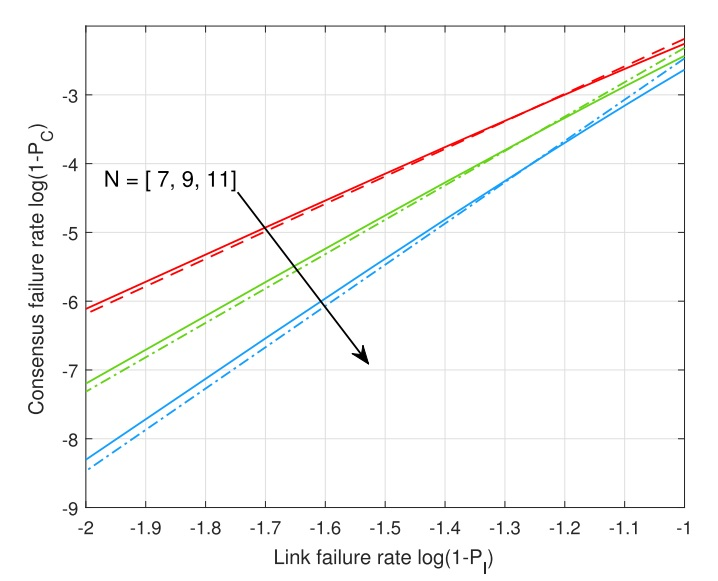
\includegraphics[scale=0.5]{eq2.jpg}
    \caption{Consensus failure rate $\log(1-P_C)$ vs. Link failure rate $\log(1-P_l)$}
\end{figure}


\end{frame}


\begin{frame}{Simulation Results}
\begin{figure}
    \centering
    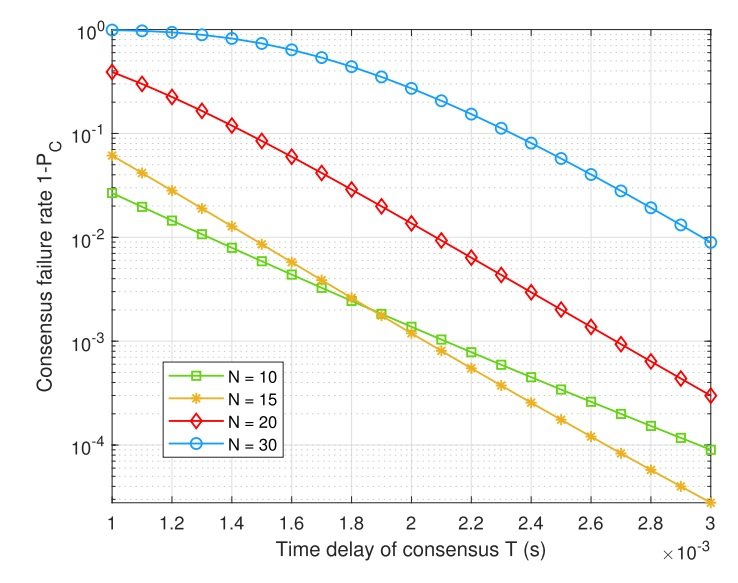
\includegraphics[scale=0.5]{eq3.jpg}
    \caption{Consensus failure rate $(1 - P_C)$ vs. Consensus delay T}
\end{figure}


\end{frame}


\begin{frame}{Simulation Results}
\begin{figure}
    \centering
    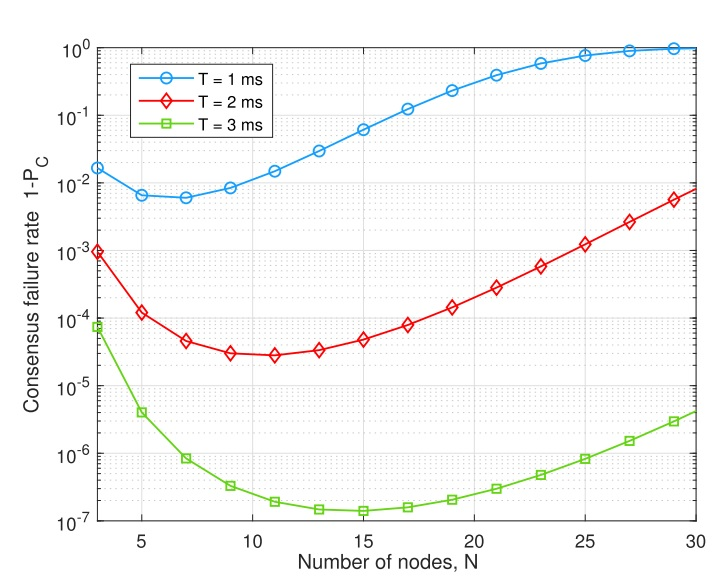
\includegraphics[scale=0.5]{eq4.jpg}
    \caption{Consensus failure rate $(1 - P_C)$ vs. Nodes number (N).}
\end{figure}

\end{frame}

\end{document}
